\section{ Valmistautuminen hyppyyn }
\label{hyppytapahtuma-valmistautuminen-hyppyyn}


Hyppytapahtuma ei suinkaan ala siitä, kun poistutaan koneesta ilmassa. Jotta kaikki sujuisi hyvin, on tärkeää huolehtia myös valmisteluista. Päätös hypätä on hyvä tehdä jo edellisenä päivänä, sillä näin ehtii henkisesti valmistautua tulevaan suoritukseen. Riittävä yöuni ja ravinto ovat myös tärkeitä – väsyneenä tai nälkäisenä keskittyminen on vaikeaa. 


Ennen hyppäämään kirjoittautumista (pokalistan täyttöä) kootaan kaikki tarvittavat varusteet ja ilmoittaudutaan hyppäämään. Varusteita on hyvä sovittaa päälle, jotta niihin voi tehdä tarvittavat säädöt ajoissa ennen koneelle lähtöä. Suoritusta harjoitellaan joko itsenäisesti tai hyppymestarin kanssa. 


Mikäli mahdollista, seuraa ennen omaa pokaasi toisten hyppääjien ohjailua varjon varassa nähdäksesi ylä- ja pintatuulien vaikutuksen ohjaamiseen ja laskeutumiseen. 


Ennen koneelle menoa hyppymestari tarkastaa, että varusteet on puettu oikein päälle. Tarkastuksen jälkeen varusteita \textbf{ei saa säätää} ilman hyppymestarin lupaa! Vallitsevan tuulen mukainen ohjauskuvio (\ref{hyppytapahtuma-laskeutumiskuvio} s.\pageref{hyppytapahtuma-laskeutumiskuvio}) käydään vielä läpi ennen koneelle menoa. Oppilaat saavat mennä koneelle vain hyppymestarin johdolla. 

\subsection{ Toiminta koneessa }
\label{hyppytapahtuma-toiminta-koneessa}


Kone kuormataan yleensä käänteisessä järjestyksessä eli se, joka menee koneeseen ensimmäisenä, hyppää viimeisenä (poikkeuksena hyppymestari). Varo varusteiden tarttumista koneessa oleviin ulokkeisiin aina koneessa liikkuessasi. Suojaa erityisesti varjojen aukaisukahvoja myös muiden liikkuessa. Jos takerrut kiinni johonkin, älä revi itseäsi irti väkisin, vaan ilmoita asiasta hyppymestarille. Vältä turhaa liikkumista. Pidä mahdolliset istuinvyöt kiinni, kunnes hyppymestari aukaisee ne tai antaa luvan aukaisuun. Ilmailumääräyksen OPS M6-1 perusteella ilma-aluksella saa kuljettaa sen päällikön ja hyppääjien suostumuksella ja omalla vastuulla enintään kymmentä hyppääjää ilman istuinvyötä.  


Jos lennon aikana huomaat omissa tai muiden varusteissa jotain poikkeavaa, ilmoita siitä heti hyppymestarille. Keskity omaan hyppyysi. Huomioi muut koneessa olijat äläkä häiritse heidän keskittymistään. Koneen päällikkö on lentäjä, mutta sinun päällikkösi on hyppymestari. Lähestyttäessä uloshyppypaikkaa kone lentää tuuliolosuhteiden perusteella määriteltyä linjaa. Hyvissä ajoin ennen uloshyppypaikkaa hyppymestari tarkastaa vielä oppilaiden varusteet. 

\section{ Uloshyppy Cessna 206, pakkolaukaisu }
\label{hyppytapahtuma-uloshyppy-cessna-206-pakkolaukaisu}


Hyppymestarin komennolla OVELLE! siirrytään (varoen repun osumista koneeseen) ovelle uloshyppyasentoon. Komennolla MENE! ponnistetaan irti koneesta, otetaan hyvä taivutus ja delta-asento sekä aletaan laskea. Rintamasuunnan on pysyttävä koko ajan suoraan koneen lentosuuntaan. 


\begin{Figure}\centering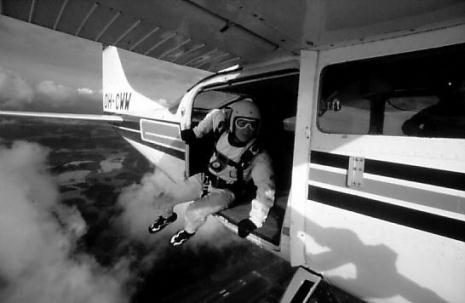
\includegraphics[width=0.7\textwidth]{206UH1.jpeg}\captionof{figure}{Hyppääjä on siirtymässä ovelle uloshyppyasentoon}\end{Figure} 


Uloshypyssä maa vetää helposti katsetta puoleensa. Jos katsoo maahan eikä koneeseen, taivutus todennäköisesti kääntyy väärin päin. Ihmisen vartalo kääntyy yleensä katseen suuntaan, joten kun uloshypyn aikana katsoo ylös koneeseen, niin vartalo on taipunut oikeanlaiselle kaarelle. Taivutus lähtee lantiosta (myös selkä ja niska). 


Tärkeintä uloshypyssä on taivutus. Delta-asennossa kädet ovat n. 45 astetta irti kyljistä, olkapäät takana. Jalat pidetään noin hartioiden levyisessä haara-asennossa ja vain hiukan koukistettuna. 


Laskeminen on tärkeää opetella heti alusta alkaen, sillä se on käytännössä ainoa tapa säilyttää ajantaju tässä vaiheessa hyppyuraa. Laskeminen tapahtuu ääneen huutamalla (101...105). Uloshyppyharjoituksissa opetellaan oikeaa rytmiä, joten ei huudeta vain numeroita vaan sekunteja. Ilmassa muutama sekunti voi tuntua hyvinkin pitkältä ajalta. 


\begin{Figure}\centering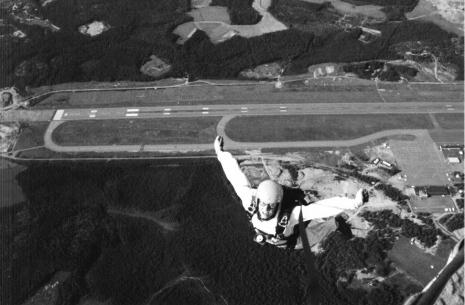
\includegraphics[width=0.7\textwidth]{206UH2.jpeg}\captionof{figure}{Hyppääjä on ponnistanut irti koneesta.}\end{Figure} 


Onnistuneen uloshypyn päätekijät ovat: 

\begin{itemize}
\item  Asettautuminen hyvään uloshyppyasentoon ovelle (katse ylös koneeseen) 
\item  Riittävä ponnistus ja rintamasuunta lentosuuntaan  
\item  Hyvä ja symmetrinen delta-asento sekä voimakas taivutus ja katse ylös koneeseen 
\end{itemize}
\section{ Uloshyppy Streevakone, pakkolaukaisu }
\label{hyppytapahtuma-uloshyppy-streevakone-pakkolaukaisu}


Hyppymestarin komennolla OVELLE! siirrytään ovelle. Komennolla MENE! siirrytään (varoen repun osumista koneeseen) roikkumaan streevalle uloshyppyasentoon, irrottaudutaan koneesta ja pidetään hyvä taivutus sekä X-asento ja aletaan laskea. Rintamasuunnan on pysyttävä koko ajan suoraan koneen lentosuuntaan. 


\begin{Figure}\centering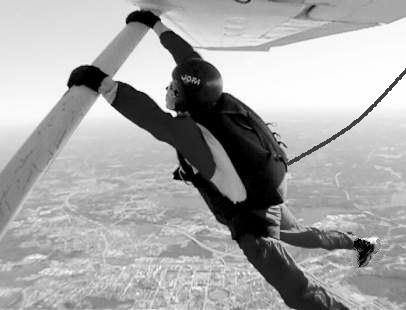
\includegraphics[width=0.7\textwidth]{Streeva-UH1.jpeg}\captionof{figure}{Hyppääjä on siirtynyt streevalle uloshyppyasentoon}\end{Figure} 


Uloshypyssä maa vetää helposti katsetta puoleensa. Jos katsoo maahan eikä koneeseen, taivutus kääntyy todennäköisesti väärin päin. Ihmisen vartalo kääntyy yleensä katseen suuntaan, joten kun katsoo uloshypyn aikana ylös kohti konetta, vartalo on taipunut oikeanlaiselle kaarelle. Taivutus lähtee lantiosta (myös selkä ja niska). 


Mikäli taivutuksesi syystä tai toisesta häviää, voit korjata tilanteen helposti: taivuttamalla. 


Tärkeintä uloshyppyasennossa ja uloshypyssä on siis taivutus. X-asennossa kädet ovat ylhäällä levitettyinä, olkapäät takana. Jalat pidetään noin hartioiden levyisessä haara-asennossa ja vain hiukan koukistettuna. 


Laskeminen on tärkeää opetella heti alusta alkaen, sillä se on käytännössä ainoa tapa säilyttää ajantaju tässä vaiheessa hyppyuraa. Laskeminen tapahtuu ääneen huutamalla (101...105). Uloshyppyharjoituksissa opetellaan oikeaa rytmiä, joten ei huudeta vain numeroita vaan sekunteja. Ilmassa muutama sekunti voi tuntua hyvinkin pitkältä ajalta. 


\begin{Figure}\centering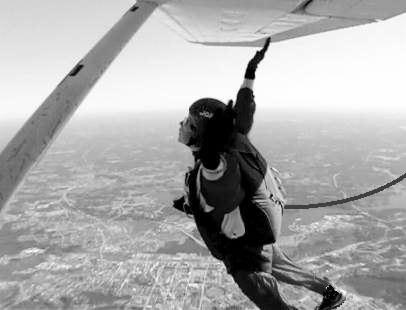
\includegraphics[width=0.7\textwidth]{StreevaUH2.jpeg}\captionof{figure}{Hyppääjä on irroittautunut koneesta.}\end{Figure} 


Onnistuneen uloshypyn päätekijät ovat: 

\begin{itemize}
\item  Asettautuminen hyvään ja symmetriseen uloshyppyasentoon (X-asento, taivutus ja katse ylös koneeseen) 
\item  Käsien yhtäaikainen irrottaminen ja rintamasuunta lentosuuntaan  
\item  Hyvä ja symmetrinen X-asento sekä voimakas taivutus ja katse ylös koneeseen 
\end{itemize}
\section{ Uloshyppy NOVA }
\label{hyppytapahtuma-uloshyppy-nova}


Hyppymestari komentaa: \textbf{SIIRRY / YLÖS} 


Siirry- tai Ylös-komennolla valmistaudut siirtymään ovelle.  


Hyppymestari komentaa: \textbf{OVELLE} 


Ovelle-komennolla hyppymestari auttaa sinua, kun siirryt ovelle (varoen repun osumista koneeseen) uloshyppyasentoon, jolloin kummatkin hyppymestarit pitävät sinusta kiinni. Tarvittaessa sisällä oleva hyppymestari antaa lisäkomentoja. 


Kun olet valmis, siirrä katseesi sisäpuolella olevaan hyppymestariin ja tee uloshyppytarkistus. Eli pidä katseesi hyppymestarissa ja sano kovalla äänellä: 


\textbf{TARKISTUS SISÄÄN} 


Tällä varmistat sisällä olevan hyppymestarin valmiuden, joka ollessaan valmis nyökkää jolloin voit jatkaa eteenpäin. Pidä katseesi hyppymestarissa niin kauan kunnes hän antaa merkin ravistamalla tai nyökkäämällä. 


Tämä jälkeen tarkista ulkona olevan hyppymestarin valmius. Siirrä katseesi olkapääsi yli ulos hyppymestariin ja sano kovalla äänellä: 


\textbf{TARKISTUS ULOS} 


Tällä varmistat ulkona olevan hyppymestarin valmiuden, joka ollessaan valmis nyökkää jolloin voit jatkaa eteenpäin. Pidä katseesi hyppymestarissa niin kauan, kunnes hän antaa merkin ravistamalla tai nyökkäämällä. 


Kun olet varmistanut hyppymestareiden valmiuden voit aloittaa rytmikkään uloshyppylaskennan ääneen. Laskenta voi vaihdella käytetyn konetyypin mukaan. 

\begin{description}
\item[\textbf{SIIPI}] \hfill \\ 
Siirrä ja pidä katseesi siivessä (tai vastaavassa kiintopisteessä) \hfill \\ 
\item[\textbf{YLÖS} (tai ULOS)] \hfill \\ 
Liikuta vartaloasi ylöspäin (tai ulospäin) \hfill \\ 
\item[\textbf{ALAS} (tai SISÄÄN)] \hfill \\ 
Liikuta vartaloasi alaspäin (tai sisäänpäin) \hfill \\ 
\item[\textbf{TAIVUTA}] \hfill \\ 
Ponnista sivuttain ulospäin, ota hyvä taivutus ja siirrä välittömästi kädet ja jalat symmetrisesti vapaapudotusasentoon. Pidä katseesi koneessa mahdollisimman pitkään koko uloshypyn ajan, sillä se edesauttaa hyvää uloshyppyä. Laske myös ääneen 105 saakka ja aloita hypyn kulku. \hfill \\ 
\end{description}

Laskeminen on tärkeää opetella heti alusta, sillä se on käytännössä ainoa tapa säilyttää ajantaju tässä vaiheessa hyppyuraa. Laskeminen tapahtuu ääneen huutamalla (101...105). Uloshyppyharjoituksissa opetellaan oikeaa rytmiä, joten ei huudeta vain numeroita vaan sekunteja. Ilmassa muutama sekunti voi tuntua hyvinkin pitkältä ajalta. 

\section{ Vapaapudotuksen perusteet }
\label{hyppytapahtuma-vapaapudotuksen-perusteet}

\begin{description}
\item[ ] \hfill \\ 
\textit{Jos olet pakkolaukaisukurssilla, voit siirtyä kohtaan: Varjon avautuminen ja lentokuntoon saattaminen, (\ref{hyppytapahtuma-varjon-avautuminen-ja-lentokuntoon-saattaminen} s.\pageref{hyppytapahtuma-varjon-avautuminen-ja-lentokuntoon-saattaminen}) ja palata tähän lukuun kun olet siirtymässä itseaukaisuhyppyihin.} \hfill \\ 
\end{description}

\begin{figure*}[]\centering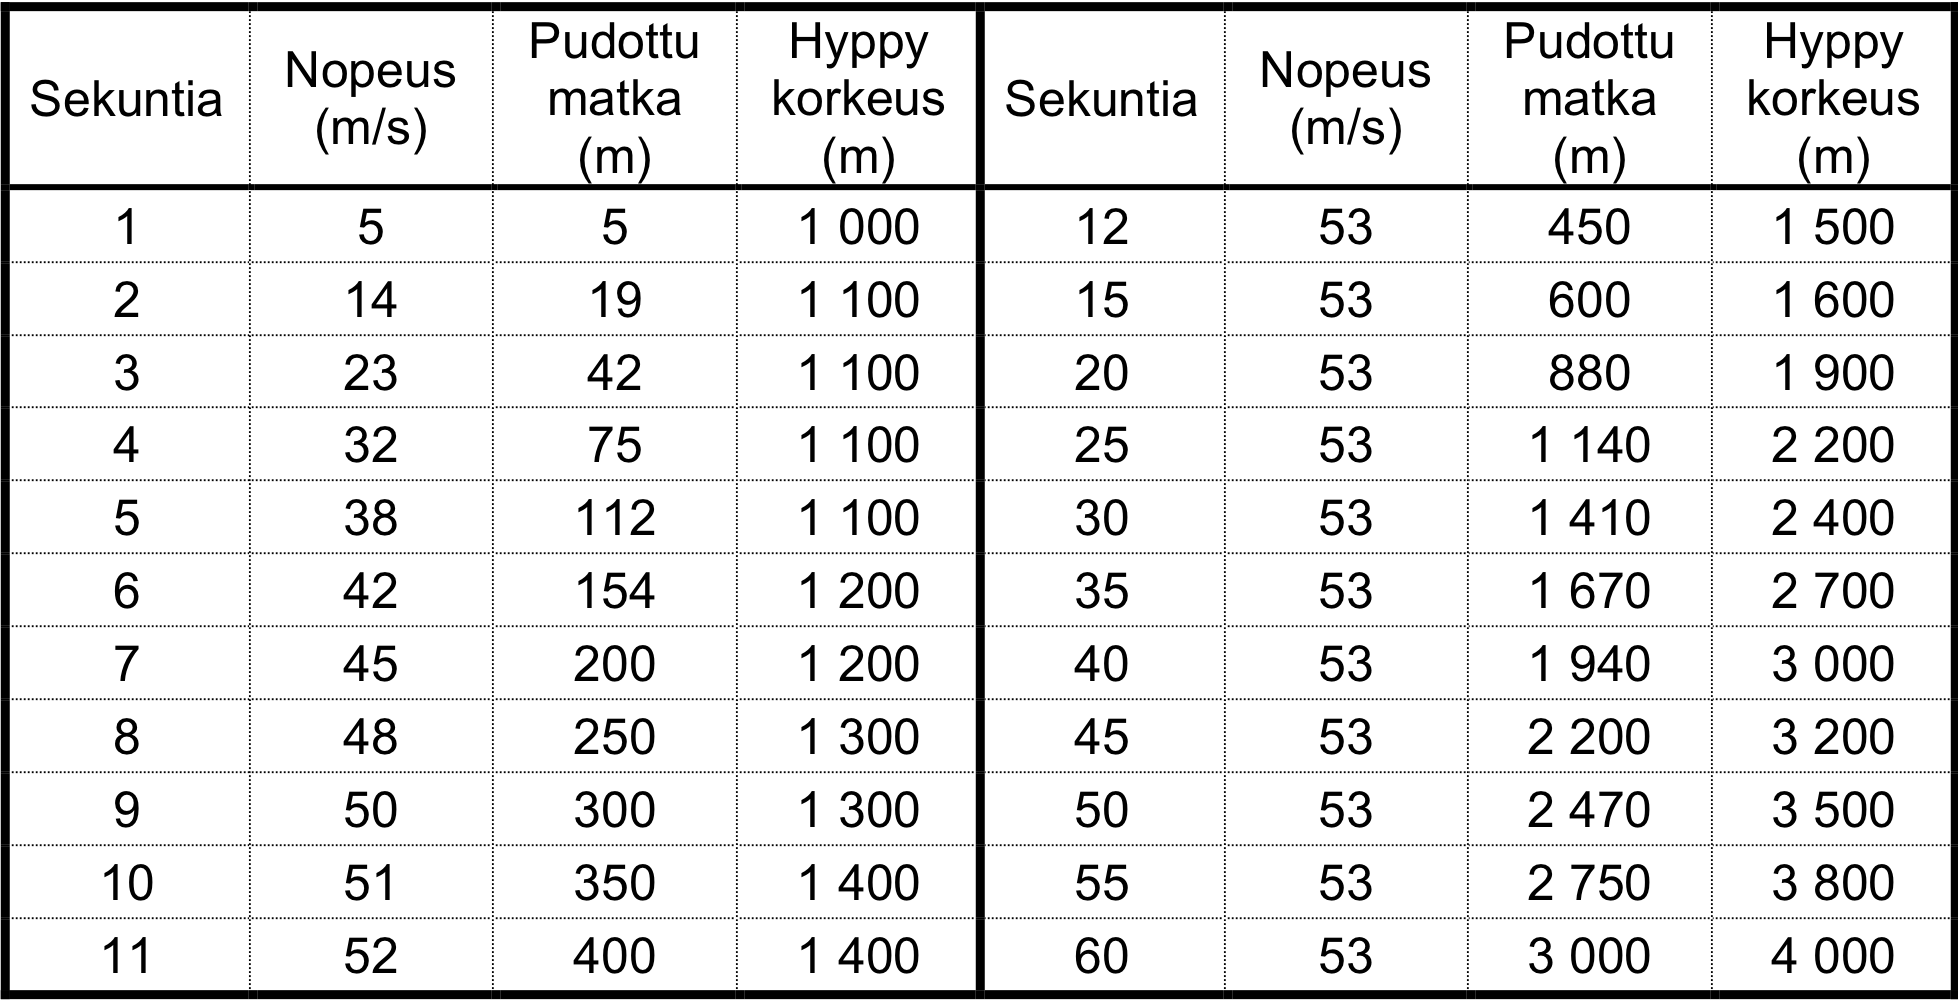
\includegraphics[width=0.7\textwidth]{Vapaapudotus-taulukko.png}\caption{Hyppääjän keskimääräinen nopeus ja pudottu matka ajan suhteen.}\end{figure*} 


Maan vetovoimasta johtuen nopeus vapaapudotuksessa kiihtyy. Ilmanvastuksen vaikutuksesta putoamisnopeudeksi vakiintuu 10–12 sekunnin kuluttua 180–190 km/h (50-53 m/s). 


Seuraavaan taulukkoon on koottuna hyppääjän keskimääräinen nopeus (maata kohti), pudottu matka hypyn alusta lähtien sekä laskennallinen hyppykorkeus, jos varjo avataan 1000 metrin korkeudessa. Putoamisnopeus riippuu mm. hyppääjän massasta, asennosta, vaatetuksesta ja hyppykorkeudesta. 


Kaikilla oppilaskoulutushypyillä varjo on avattava aina viimeistään 1000 metrin korkeudessa. Jos avaus jostain syystä tapahtuu alle 800 metrin korkeudessa, on asiasta ilmoitettava heti kouluttajalle. Jos käytössä on FXC-12000-automaattilaukaisin, on se todennäköisesti herkistynyt ja saattaa seuraavalla hypyllä avata varavarjon virheellisesti. 

\subsection{ Korkeusmittarin käyttö vapaassa }
\label{hyppytapahtuma-korkeusmittarin-kaytto-vapaassa}


\begin{figure*}[]\centering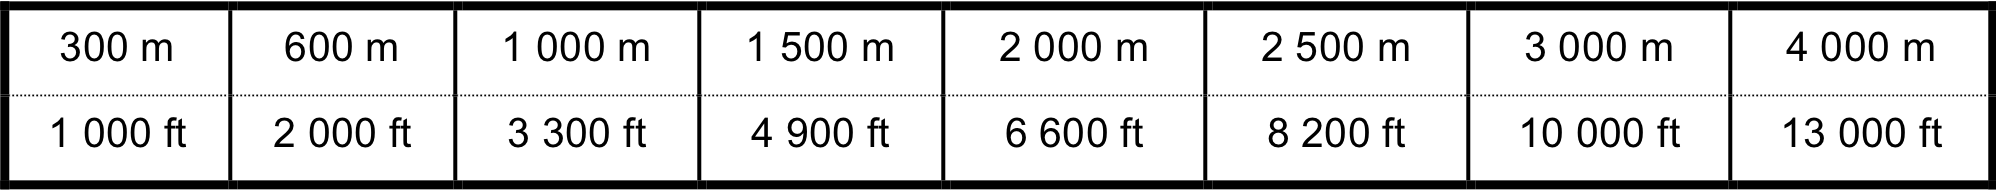
\includegraphics[width=0.8\textwidth]{Metrit-jaloiksi-taulukko.png}\caption{Nämä pyöristetyt muunnokset tulee osata hyppytoiminnassa.}\end{figure*} 


Kaikilla laskuvarjohypyillä on käytettävä visuaalista korkeusmittaria. Poikkeuksena ovat vesihypyt, joilla hyppykorkeus ei ylitä 1500 metriä. Mittarit perustuvat ilmanpaineen muutokseen. Ilmanpaine pienenee noin 1 mbar / 8 m ylöspäin mentäessä.  


Pakkolaukaisukurssin käyneet oppilaat alkavat harjoitella mittarin käyttöä 5 sekunnin vapaapudotushypystä lähtien. Ensin mittarin käyttöön totutellaan laskemisen määrätessä varjon avaushetken. Jo 10 sekunnin vapaapudotushypyllä on laskeminen vain varmistuskeino toimivan mittarin määritellessä avauskorkeuden. Seuraa korkeutta jatkuvasti noin viiden sekunnin välein. 


Korkeusmittarit jaetaan kahteen pääryhmään, visuaalisiin ja äänikorkeusmittareihin. Visuaalisesta mittarista luetaan hyppykorkeus, purku- ja avauskorkeus, päätöskorkeus varavarjotilanteessa sekä ohjaamiseen liittyvät korkeudet. Äänikorkeusmittarit hälyttävät ennalta asetetussa korkeudessa tai korkeuksissa.  


Visuaalinen, metriasteikolla varustettu osoitinmittari, on ainoa hyväksyttävä mittari hyppyuran alussa.   


Visuaalisessa korkeusmittarissa on 

\begin{itemize}
\item  näyttöväli 10, 50 tai 100 metriä ja numerot 100 tai 500 metrin välein. 
\item  avauskorkeus 800 tai 1000 metriä merkitty eri värillä. 
\item  joko osoitinmittari tai digitaalinen, jossa numeronäyttö. 
\end{itemize}

Mittarin näyttöasteikko voi osoittaa korkeuden joko metreinä tai jalkoina (feet = ft). Jalka = 0,3048 m. 

\subsection{ Käyttö }
\label{hyppytapahtuma-kaytto}


Korkeusmittaria käytettäessä on huomioitava seuraavat asiat: 

\begin{itemize}
\item  Mittari on asetettava paikkaan, josta se nähdään aina. 
\item  Perusasennon on säilyttävä mittaria katsottaessa. 
\item  Mittaria vilkaistaan päätä kääntämällä tai FS-hypyillä voidaan katsoa myös muiden mittareita. 
\item  Mittaria luetaan vertaamalla viisarin asentoa punaisen alkuun eikä numeroihin tuijottamalla. 
\item  Ajantajun on säilyttävä jokaisella hypyllä, sillä mittari voi mennä rikki.  
\item  Mittarin jumiutuessa, tai jos mittari ei ole luettavissa, avataan varjo heti, mutta huomioidaan kuitenkin muut hyppääjät. 
\item  Freehypyillä suositellaan käsimittaria. Ensimmäisillä freehypyillä kannattaa käyttää myös rintamittaria. 
\item  Käytettäessä integraalikypärää suositellaan käsimittaria, sillä rintamittari ei ole välttämättä luettavissa. 
\item  Mittarit on kalibroitu toimimaan tarkimmin avauskorkeusalueella. Korkealla esiintyvät näyttöerot ovat tavallisia.  
\end{itemize}
\subsection{ Virheet }
\label{hyppytapahtuma-virheet}


Yleisimmät viat ja virheet korkeusmittarin toiminnassa ovat: 

\begin{itemize}
\item  paine-erot ja virhenäytöt vapaapudotushypyillä esimerkiksi käytettäessä rintamittaria selkälennossa 
\item  mittarin jäätyminen kosteuden tai tiivistyneen veden takia 
\item  jumiutuminen iskujen tai lian takia 
\item  mekaaninen vika, joka aiheutuu mittarin pudotessa maahan tai maassa olevan mittarin päälle astumisesta 
\item  paristojen loppuminen 
\end{itemize}

Korkeuserojen laskeminen ja mittariasetus on osattava, jos lähtö- ja alastulopaikka eivät ole samat. 


\end{multicols}\pagebreak\begin{multicols}{2} 

\section{ Avaaminen }
\label{hyppytapahtuma-avaaminen}

\subsection{ Avauksen tärkeysjärjestys }
\label{hyppytapahtuma-avauksen-tarkeysjarjestys}

\begin{framed}
\begin{enumerate}[label=\bfseries \arabic*)]
\item  \textbf{Avaa varjo.} Itseaukaisuhypyllä tärkein tehtäväsi on aina avata itse varjosi. 
\item  \textbf{Avaa avauskorkeudessa} Jokaiselle hypyllä on aina määrätty avauskorkeus, jossa varjo on ehdottomasti avattava. 
\item  \textbf{Avaa stabiilissa asennossa} Pyri avaamaan varjosi stabiilissa asennossa, mutta tärkeämpää on avata oikeassa korkeudessa. 
\end{enumerate}
\end{framed}

\subsection{ Avausjärjestelmät }
\label{hyppytapahtuma-avausjarjestelmat}

\subsubsection{ Jousiapuvarjo  }
\label{hyppytapahtuma-jousiapuvarjo}


Jousikuormitettu apuvarjo kiinnitetään yhdyspunoksella sisäpussin kautta päävarjoon. Jousi on malliltaan joko kartion muotoinen tai tasapaksu. Jousiapuvarjo on kokonaan F-111-kangasta tai valmistettu osittain harsokankaasta. Jousiapuvarjo on alaosastaan avonainen tai suljettu. Jousiapuvarjolla avaaminen tapahtuu vetämällä avauskahvasta. Pidä kahva kädessäsi ja laita se talteen avauksen jälkeen. 

\subsubsection{ Kädestä päästettävä apuvarjo (HD) }
\label{hyppytapahtuma-kadesta-paastettava-apuvarjo-hd}


Avattaessa HD-avausjärjestelmällä apuvarjo heitetään reippaasti puhtaaseen ilmavirtaan. Kädestä päästettävän apuvarjon heittäminen käännöksen tai lattakierteen aikana aiheuttaa aina avautumisongelmia, kuten kierrettä. Jos avausasento ei ole stabiili, jää HD-apuvarjo myös helpommin kiinni hyppääjän varusteisiin ja raajoihin.  


Jousiapuvarjolla aloittaneen oppilaan pitää saada koulutus siirtyessään HD-apuvarjoon. Koulutuksen jälkeen on osattava HD-apuvarjon heittäminen vapaaseen ilmatilaan hyppääjän aiheuttamien pyörteiden ulkopuolelle. Vähintään ensimmäisellä HD-hypyllä (HD-totuttelu) ei tehdä muita suorituksia. HD-totuttelun jälkeen ei pitäisi palata enää kahvavetoisiin varusteisiin. 


\begin{Figure}\centering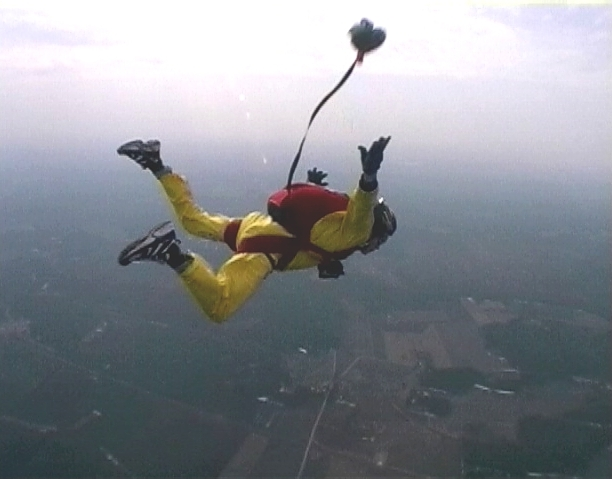
\includegraphics[width=0.8\textwidth]{HD-apuvarjo.jpeg}\captionof{figure}{Hyppääjä on heittänyt HD-apuvarjon ja on palauttamassa käsiään perusasentoon}\end{Figure} 

\subsection{ Vaaratilanteet }
\label{hyppytapahtuma-vaaratilanteet}

\begin{itemize}
\item  Epästabiili asento, kädet/käsi tai jalat/jalka sisällä ⇨ kaatuu kyljelleen/selälleen ⇨ mahdollista sotkeutua avautuvaan varjoon. 
\item  Veto irtipäästöpampulasta ⇨ päävarjo irtoaa normaalin avauksen jälkeen ⇨ tehdään varavarjotoimenpiteet. 
\item  Veto varavarjon kahvasta ⇨ varavarjo aukeaa. 
\item  Veto valjaista / kahva ei lähde / ei vetoa ⇨ päävarjo ei aukea ⇨ uusitaan veto tai tehdään varavarjotoimenpiteet. 
\item  Apuvarjo tarttuu kiinni hyppääjään ⇨ yksi irrotusyritys, jos nähtävissä ⇨ aukeaa tai varavarjotoimenpiteet. 
\item  Punokset sotkeutuvat hyppääjään ⇨ pyritään irrottautumaan sotkeutuneista punoksista, käytetään tarvittaessa koukkupuukkoa ⇨ tehdään varavarjotoimenpiteet. 
\item  Apuvarjo voi avauksessa joskus tulla kuvun etureunan kautta kuvun alapuolelle ⇨ tehdään ohjauskokeilu ⇨ jos varjo ei käyttäydy normaalisti, tehdään varavarjotoimenpiteet.  
\item  Asento hallitsematon ⇨ avataan päävarjo heti. 
\item  Apuvarjo turbulenssissa: 
\end{itemize}

Avauksessa apuvarjo voi jäädä hyppääjän selän taakse muodostuvaan pyörteeseen eli turbulenssiin. Jos vedon jälkeen 105:n kohdalla ei ole tapahtunut mitään, vilkaistaan olkapään yli. Asento kallistuu ja apuvarjon pitäisi saada ilmaa. Ellei varjo avaudu, tehdään varavarjotoimenpiteet, koska apuvarjo tai yhdyspunos on saattanut tarttua johonkin kiinni tai reppu on jumissa. Kiinnitarttumista voidaan yrittää irrottaa, jos varmuudella nähdään ongelman aiheuttaja. Jos irrotus ei onnistu yhdellä yrityksellä tai ongelman aiheuttajaa ei nähdä, tehdään varavarjotoimenpiteet heti. 


\begin{Figure}\centering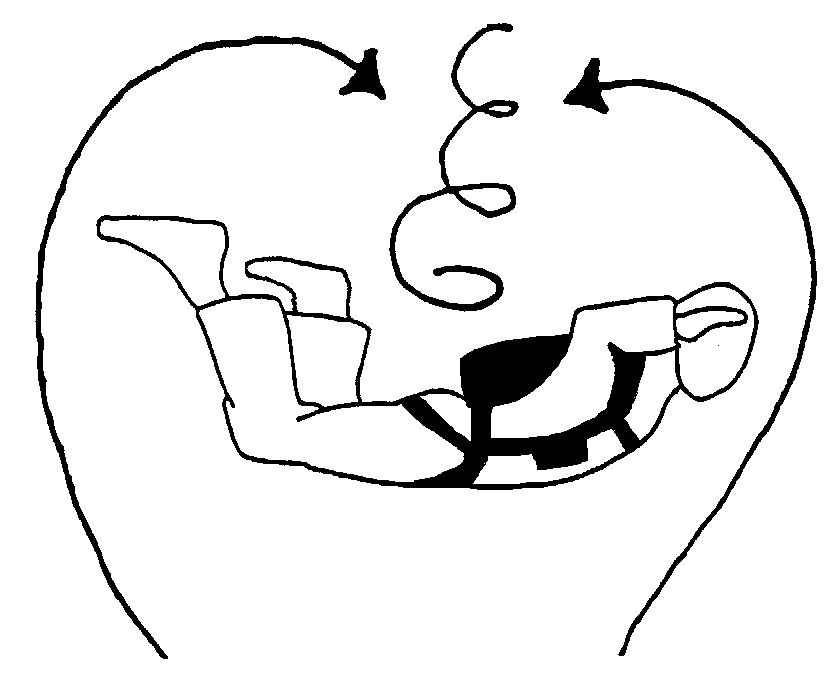
\includegraphics[width=0.7\textwidth]{Selka-turbulenssi.png}\captionof{figure}{Hyppääjän selän taakse muodostuu turbulenssi}\end{Figure} 

\section{ Varjon avautuminen ja lentokuntoon saattaminen }
\label{hyppytapahtuma-varjon-avautuminen-ja-lentokuntoon-saattaminen}


Pakkolaukaisujärjestelmässä koneesta irtautuessa pakkolaukaisujärjestelmä ja vastaavasti NOVA:ssa ilmavirtaan heitetty apuvarjo avaa päävarjon repun jonka jälkeen avausjärjestelmä vetää sisäpussin ulos repusta. Punokset alkavat purkautua kumilenkeistään. Kupu tulee ulos sisäpussista ja alkaa kehittyä keskeltä. Slider liukuu punoksia pitkin alas hidastaen kuvun aukeamista. Sinun tehtäväksesi jää varjon tarkastaminen ja sen lopullinen avaaminen. 


Kun olet päässyt laskemisessa 105:een, tarkasta varjo. Varjo LENTÄÄ, kun 

\begin{itemize}
\item  Kupu on säännöllisen muotoinen 
\item  Punokset ovat kireällä 
\item  Slider on suorakaiteen muotoinen. 
\end{itemize}

Tarkastettuasi varjon vie kädet takimmaisille kantohihnoille. Jos punokset ovat kierteellä, avaa ne potkimalla ja levittämällä kantohihnoja (SELVITÄ). 


Vedä molemmista ohjauslenkeistä (sijaitsevat takimmaisten kantohihnojen takapuolella) alaspäin avataksesi puolijarrut. Puolijarrut saat avata vasta kierteiden poiston jälkeen.  


Tarvittaessa pumppaa slider alas ja tunnelit auki. Pumppaus tehdään vetämällä ohjauslenkit rauhallisesti muutamaksi sekunniksi noin vyötärön tasolle ja palauttamalla ohjauslenkit sitten rauhallisesti takaisin yläasentoon. Pumppauksen voit toistaa useampia kertoja (SELVITÄ).  


Mikäli varjo EI LENNÄ tai EI SELVIÄ, siirry välittömästi varavarjotoimenpiteisiin. (\ref{paavarjon-vajaatoiminnot-varavarjon-kaytto} s.\pageref{paavarjon-vajaatoiminnot-varavarjon-kaytto}) 


Kun olet suorittanut varjon lopullisen avaamisen, tarkasta seuraavat asiat: 

\begin{framed}
\begin{itemize}
\item  ILMATILA (myös kierteiden avauksen ja pumppauksen aikana, väistä tarvittaessa ja/tai varoita huutamalla (\ref{mahdolliset-vaaratilanteet-tormaaminen-varjon-varassa} s.\pageref{mahdolliset-vaaratilanteet-tormaaminen-varjon-varassa})) 
\item  KORKEUS (myös kierteiden avauksen ja pumppauksen aikana) 
\item  KAHVAT taskuissaan (varavarjon kahva ja päävarjon irtipäästöpampula) 
\item  SIJAINTI (oma ja maalialueen sijainti) 
\end{itemize}
\end{framed}

Aloita ohjaaminen ja käännä varjo tarvittaessa vastatuuleen. 


\end{multicols}\pagebreak\begin{multicols}{2} 

\section{ Ohjaaminen }
\label{hyppytapahtuma-ohjaaminen}

\subsection{ Lentotilat }
\label{hyppytapahtuma-lentotilat}

\begin{description}
\item[Täysliito: ] \hfill \\ 
Nosta ohjauslenkit täysin ylös. Varjo saavuttaa suurimman vaakanopeuden ja lentää parhaiten vastatuuleen. \hfill \\ 
\item[Puolijarrutustila: ] \hfill \\ 
Vedä/nosta ohjauslenkit hartioiden korkeudelle. Varjo jarruttaa.  \hfill \\ 
\item[Täysjarrutus: ] \hfill \\ 
Vedä ohjauslenkit noin lantion tasalle. Varjo jarruttaa voimakkaasti. \hfill \\ 
\item[Sakkaus:] \hfill \\ 
Jos ohjauslenkkejä painetaan vielä täysjarrutustilaa alemmaksi, varjo lakkaa lentämästä. Sakkauksessa varjon vajoamisnopeus kasvaa, joten varo sakkaamasta varjoasi matalalla. Varjo palautetaan sakkaustilasta nostamalla ohjauslenkkejä rauhallisesti 10–20 cm. Tämän jälkeen tarkasta varjo ja selvitä sitä tarpeen mukaan. (\ref{paavarjon-vajaatoiminnot} s.\pageref{paavarjon-vajaatoiminnot}) \hfill \\ 
\end{description}

Kokeile varjon eri lentotiloja, mutta muista, että kaikki ohjauskokeilut tulee tehdä yli 600 metrissä. 

%% \end{multicols}{2}
%% \begin{multicols}{2}

\begin{Figure}\centering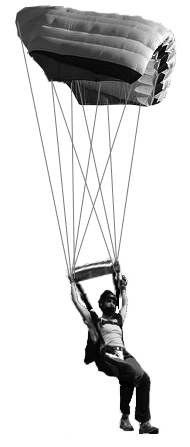
\includegraphics[width=0.5\textwidth]{Lentotila-taysi.jpeg}\captionof{figure}{Täysliito}\end{Figure} \begin{Figure}\centering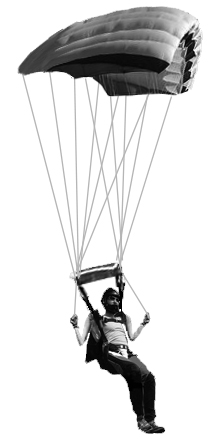
\includegraphics[width=0.5\textwidth]{Lentotila-puoli.jpeg}\captionof{figure}{Puolijarrutus}\end{Figure} 
\begin{Figure}\centering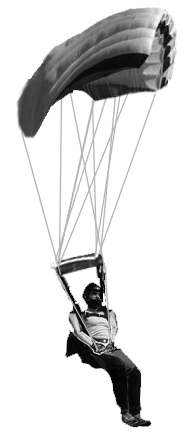
\includegraphics[width=0.5\textwidth]{Lentotila-jarru.jpeg}\captionof{figure}{Täysjarrutus}\end{Figure} 

\subsection{ Ilma- ja maanopeus }
\label{hyppytapahtuma-ilma-ja-maanopeus}


Liitovarjo on hyvin turvallinen, mutta se voi olla suuren suorituskykynsä takia väärin käytettynä hyppääjälle vaarallinen. On tärkeää tietää varjon ominaisuudet ja hallita oikea käyttötapa. 


Liitovarjo lentää ilmassa aina samaa nopeutta täysliidossa (noin 8-10 m/s) tuulista riippumatta. Tätä vakionopeutta kutsutaan ilmanopeudeksi, johon ei vaikuta se, lennetäänkö myötä\mbox{-,} sivu- vai vastatuuleen. Maanopeus on nopeus, jolla varjo liikkuu maahan nähden. Maanopeus muuttuu riippuen siitä, mihin suuntaan tuuleen nähden lennetään. Liitovarjo liikkuu maahan nähden nopeammin myötätuuleen kuin vastatuuleen. Tämän takia liitovarjolla pyritään aina laskeutumaan vastatuuleen. 


\begin{figure*}[]\centering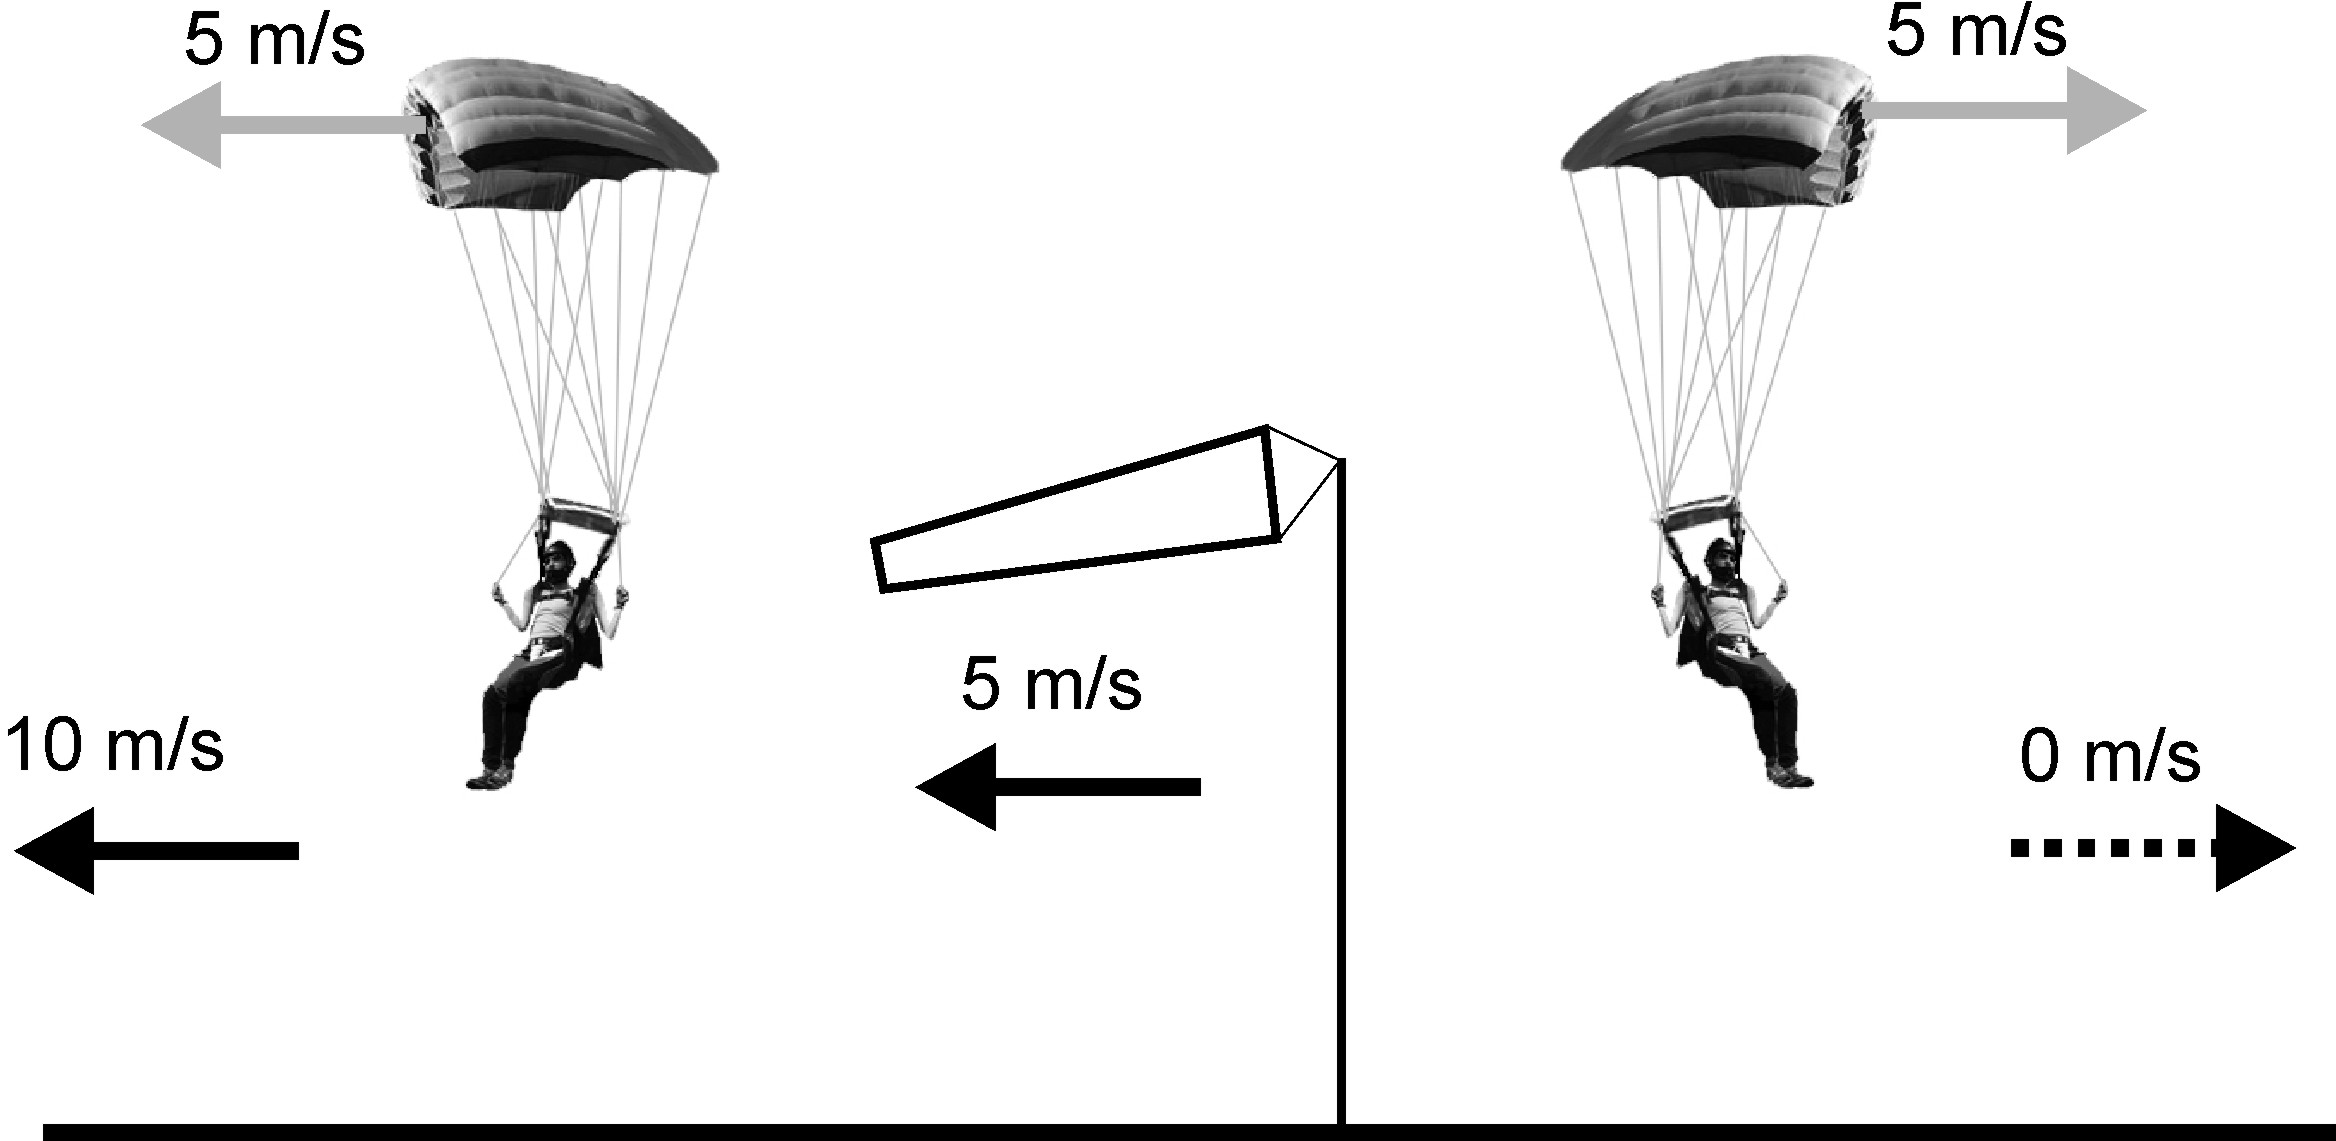
\includegraphics[width=0.7\textwidth]{Ilma-ja-maanopeus.jpeg}\caption{Maanopeus muuttuu riippuen siitä, mihin suuntaan tuuleen nähden lennetään.}\end{figure*} 

\subsection{ Turbulenssi }
\label{hyppytapahtuma-turbulenssi}


\begin{figure*}[]\centering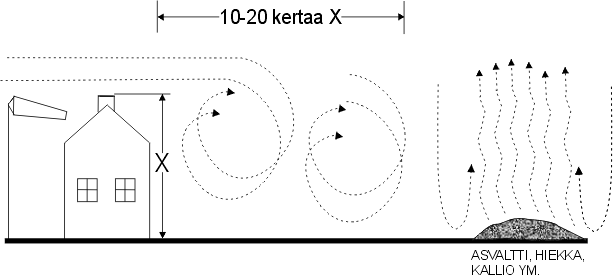
\includegraphics[width=0.7\textwidth]{Turbulenssi.png}\caption{Rakennukset ja lämmin maa aiheuttavat turbulenssia}\end{figure*} 


Turbulenssi ja epätasaiset ilmavirtaukset voivat muuttaa tunneleihin kohdistuvan virtauksen suuntaa siten, että varjo menettää kantokykynsä. Voimakas turbulenssi voi tyhjentää kuvun osittain tai jopa kokonaan. Tyhjentynyt kupu täyttyy uudestaan, kun kupu saavuttaa oikean kohtauskulman ilmavirtaan nähden. Turbulenttinen sää voi estää hyppäämisen, vaikka tuulen voimakkuus ei ylittäisikään oppilastoiminnan tuulirajaa. Jos joudut varjon varassa turbulenssiin, lennä täydessä liidossa. Liian suurilla jarruilla lentäminen saattaa aiheuttaa kuvun sakkaamisen pyörteen vaikutuksesta. 


Pyörre eli turbulenssi voi olla minkä kokoinen tahansa. Pyörteet ovat halkaisijaltaan muutamasta metristä kymmeniin metreihin. Pyörteet syntyvät ilman vapaan virtauksen rikkovista esteistä, kuten rakennuksista, puista, kukkuloista ja maaston lämpötilaeroista (nousevat ja laskevat ilmavirtaukset). Myös toisen laskuvarjon taakse ilmassa muodostuu turbulenssi. 


Hyppääjälle vaarallisimpia ovat yleensä esteistä ja nousevista tai laskevista ilmavirtauksista johtuvat pyörteet. Pyörteitä voi välttää laskeutumalla tarpeeksi kauas esteistä ja esimerkiksi hiekan reunasta, jossa virtausten suunnat muuttuvat. 

\subsection{ Käännökset }
\label{hyppytapahtuma-kaannokset}


Vasemmasta ohjauslenkistä vetämällä varjo kääntyy vasemmalle ja oikeasta vetämällä vastaavasti oikealle. Varjo kallistuu käännöksen suuntaan, joten myös vajoamisnopeus kasvaa. Tämän takia matalalla \textbf{ei saa} tehdä jyrkkiä käännöksiä. 


Käännökset täysliidosta vaativat suuren lentonopeuden takia suuren kääntösäteen. Varjo kallistuu käännöksessä sitä enemmän, mitä enemmän toista ohjauslenkkiä painetaan alaspäin. Tällöin myös vajoaminen kiihtyy. 


Käännökset puolijarrutuksesta tehdään pitämällä toinen ohjauslenkki hartioiden tasalla ja painamalla toista alemmaksi. Varjo kääntyy nopeammin mutta ei kallistu niin paljon. Vajoaminen ei ole niin voimakasta kuin täysliitokäännöksessä. 


Käännökset täysjarrutuksesta tehdään nostamalla vastakkaista ohjauslenkkiä. Varjo reagoi nopeasti ja kallistuu vähemmän kuin muissa lentotiloissa. Täysjarrutustilassa kupu on lähellä sakkaustilaa, joten käännökset on tehtävä hyvin varovasti. 


Mitä suurempi varjon lentonopeus on käännöksessä, sitä suurempi on myös varjon vajoamisnopeus ja kääntösäde. 


Kokeile varjon käyttäytymistä, älä pelkää ohjata sitä. 

\subsection{ Ohjaaminen laskeutumisalueelle }
\label{hyppytapahtuma-ohjaaminen-laskeutumisalueelle}


\begin{figure*}[]\centering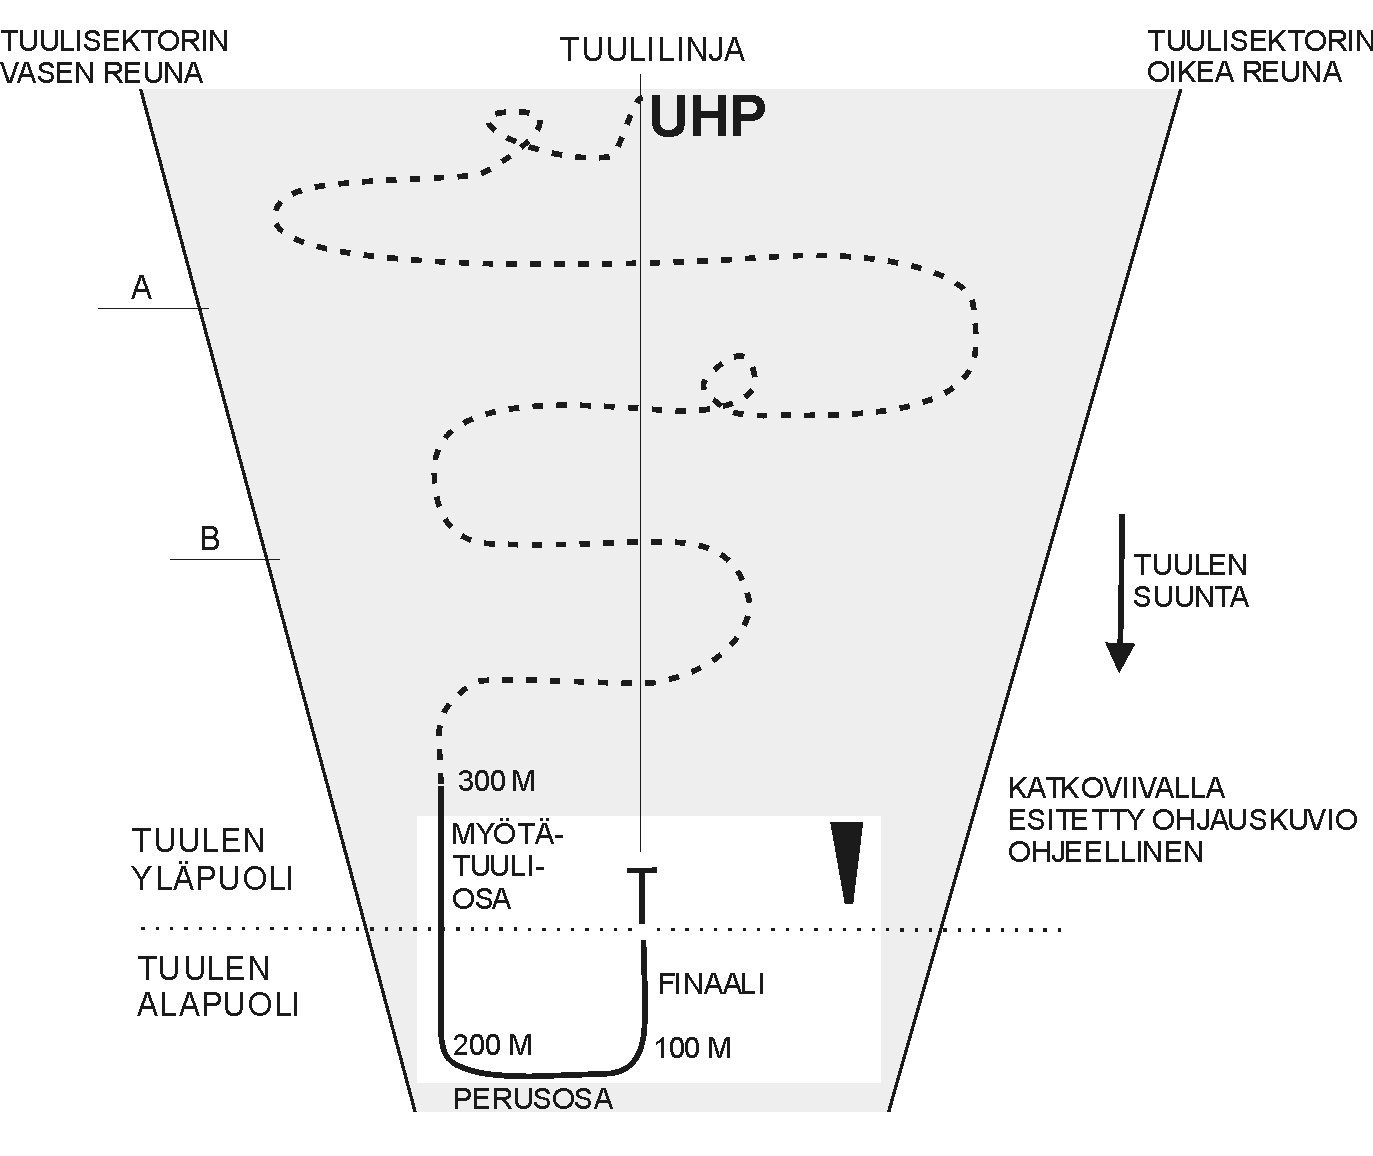
\includegraphics[width=0.5\textwidth]{Tuulisektori.png}\caption{Pysy tuulisektorilla lähestyessäsi laskeutumisaluetta.}\end{figure*} 


Tarkastettuasi ilmatilan, korkeuden, kahvat ja sijainnin aloita ohjaaminen ja käännä varjo tarvittaessa vastatuuleen, jotta pysyt suunnitellulla tuulisektorilla etkä ajaudu liian aikaisin maalialueen lähelle. Vedä mielessäsi viiva nykyisestä paikastasi loppukuvioiden aloituskohtaan ja aseta sille muutama välietappi (kuvassa A ja B). Pudota korkeutta riittävästi ennen seuraavalle välietapille siirtymistä, tarvittaessa lennä hetki vastatuuleen jotta et lähesty sitä liian aikaisin. Selvitä myös sektorin sivurajat, joita et ylitä. Kokeile tämän jälkeen varjon käyttäytymistä eri lentotiloissa: täysliito, puolijarrutus, täysjarrutus ja käännökset. Harjoittele myös loppuvetoa. Lähesty laskeutumisaluetta ottaen huomioon tuuliolosuhteet ja em. lähestymispisteet. Viimeisen 300 metrin matkalla suoritat laskeutumiskuvion, johon kuuluu kolme osaa: myötätuuliosa, perusosa ja finaali. Säännöllisin osuus on finaali, muut osuudet riippuvat tuuliolosuhteista. Tuulisektori on ilmatilakaistale, jossa pysymällä pääset laskeutumaan maalialueelle. Se sijaitsee tuulilinjan molemmin puolin. Oikean uloshyppypaikan ja maalipisteen välinen linja on tuulilinja, pysy sen läheisyydessä. Mitä lähempänä maalialuetta lennetään, \mbox{sitä kapeampi on tuulisektori.} 


\subsection{ Laskeutumiskuvio }
\label{hyppytapahtuma-laskeutumiskuvio}


Laskeutumiskuvio kannattaa lentää varjo puolijarrutuksessa. Puolijarrutustilassa lennettäessä maanopeus on pienempi, varjo kääntyy nopeammin sekä vajoaa käännöksissä vähemmän kuin täysliidossa. 


Myötätuuliosa aloitetaan 300 metrin korkeudessa tuulen yläpuolelta (aloituspiste riippuu tuulen voimakkuudesta). Myötätuuliosa lennetään tuulen alapuolelle noin 100 metriä maalipisteen sivussa. Tuulen alapuolelle lennettävä matka riippuu maatuulen voimakkuudesta.  


Perusosa on sivutuuleen lennettävä osuus. Myötätuuliosalta käännytään perusosalle noin 200 metrin korkeudella. Perusosalla lennetään suoraan maalipisteen taakse tuulen alapuolella. Mitä kovempi tuuli on, sitä enemmän on pidettävä varjoa kääntyneenä vastatuulen suuntaan päästäkseen perusosalla maahan nähden suoraan sivutuuleen. Jos aloitat perusosan liian matalalla, voit oikaista reittiäsi niin, että finaali jää lyhyemmäksi. Vastaavasti, jos aloitat perusosan liian korkealla, voit koukata hieman kauempaa jotta saat aloitettua finaalin haluamassasi pisteessä. 


\begin{Figure}\centering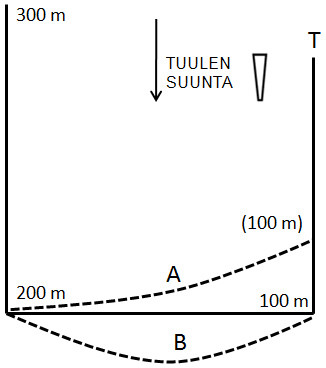
\includegraphics[width=0.8\textwidth]{Laskeutumiskuvio.png}\captionof{figure}{Jos ollaan liian matalalla, voidaan lentää reittiä A. Jos korkeutta on liikaa, voidaan lentää reittiä B.}\end{Figure} 


Vastatuuliosa eli finaali aloitetaan suoraan maalipisteen takaa tuulen alapuolelta. Aloituspiste muuttuu tuulen voimakkuudesta riippuen. Kovalla tuulella finaalin aloituspiste on lähempänä maalipistettä. Finaaliin, joka siis lennetään vastatuuleen, käännytään 100 metrin korkeudessa. Varjo saattaa pyrkiä kääntymään, joten sitä tulee \textbf{ohjata maahan asti}, jotta se pysyisi tarkasti vastatuulessa.  


Jos huomaat lentäväsi finaalissa myötätuuleen, älä käänny vastatuuleen vaan \textbf{laskeudu myötätuuleen}. Myötä- tai sivutuuleen laskeutuminen on turvallisempaa kuin käännöksessä maahan osuminen! 


S-mutkia koko laskeutumiskuvion aikana tulee välttää. Lennä niin, että muut pystyvät ennakoimaan lentoratasi. Tarkkaile ilmatilaa myös laskeutumiskuviossa. 

\begin{verbatim}        
\end{verbatim}

\begin{Figure}\centering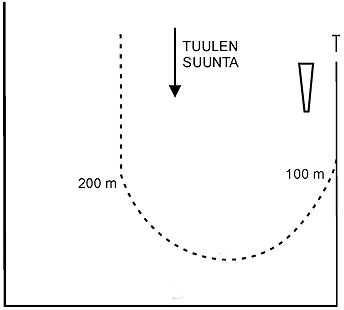
\includegraphics[width=0.8\textwidth]{Laskeutumiskuvio-kovatuuli.png}\captionof{figure}{Kovalla tuulella myötätuuliosuus aloitetaan kauempaa ja loppukuviot lennetään lähempänä maalia. Perusosa jää lyhyemmäksi. (katkoviiva)}\end{Figure} 

\subsection{Laskeutumisen tärkeysjärjestys}
\label{hyppytapahtuma-laskeutumisen-tarkeysjarjestys}

\begin{framed}
\begin{enumerate}[label=\bfseries \arabic*)]
\item  \textbf{Suora finaali} (tärkeintä on, ettei varjo ole laskeuduttaessa käännöksessä) 
\item  Tee \textbf{loppuveto} aina vähintään puolijarrutustilaan 
\item  Pyri laskeutumaan \textbf{vastatuuleen}, esteettömälle alueelle 
\end{enumerate}
\end{framed}

Muista aina laskeutumisen tärkeysjärjestys, se auttaa sinua laskeutumaan turvallisesti! 

\subsection{ Loppuveto ja maahantulo  }
\label{hyppytapahtuma-loppuveto-ja-maahantulo}


Ollessasi finaalissa noin 50 metrin korkeudessa ota hyvä alastuloasento: 

\begin{itemize}
\item  Kädet ohjauslenkeissä 
\item  Leuka kiinni rinnassa ja hampaat yhdessä 
\item  Polvet joustavasti hiukan koukussa ja \textbf{tiukasti} yhdessä 
\item  Jalkaterät 45° etenemissuunnasta sivulle ja \textbf{tiukasti} yhdessä 
\item  Jalkapohjat samalla tasolla ja maanpinnan suuntaiset. 
\end{itemize}

\begin{Figure}\centering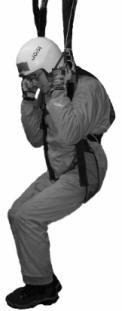
\includegraphics[width=0.5\textwidth]{Alastuloasento.jpeg}\captionof{figure}{Alastuloasento ennen loppuvetoa}\end{Figure} \begin{figure*}[]\centering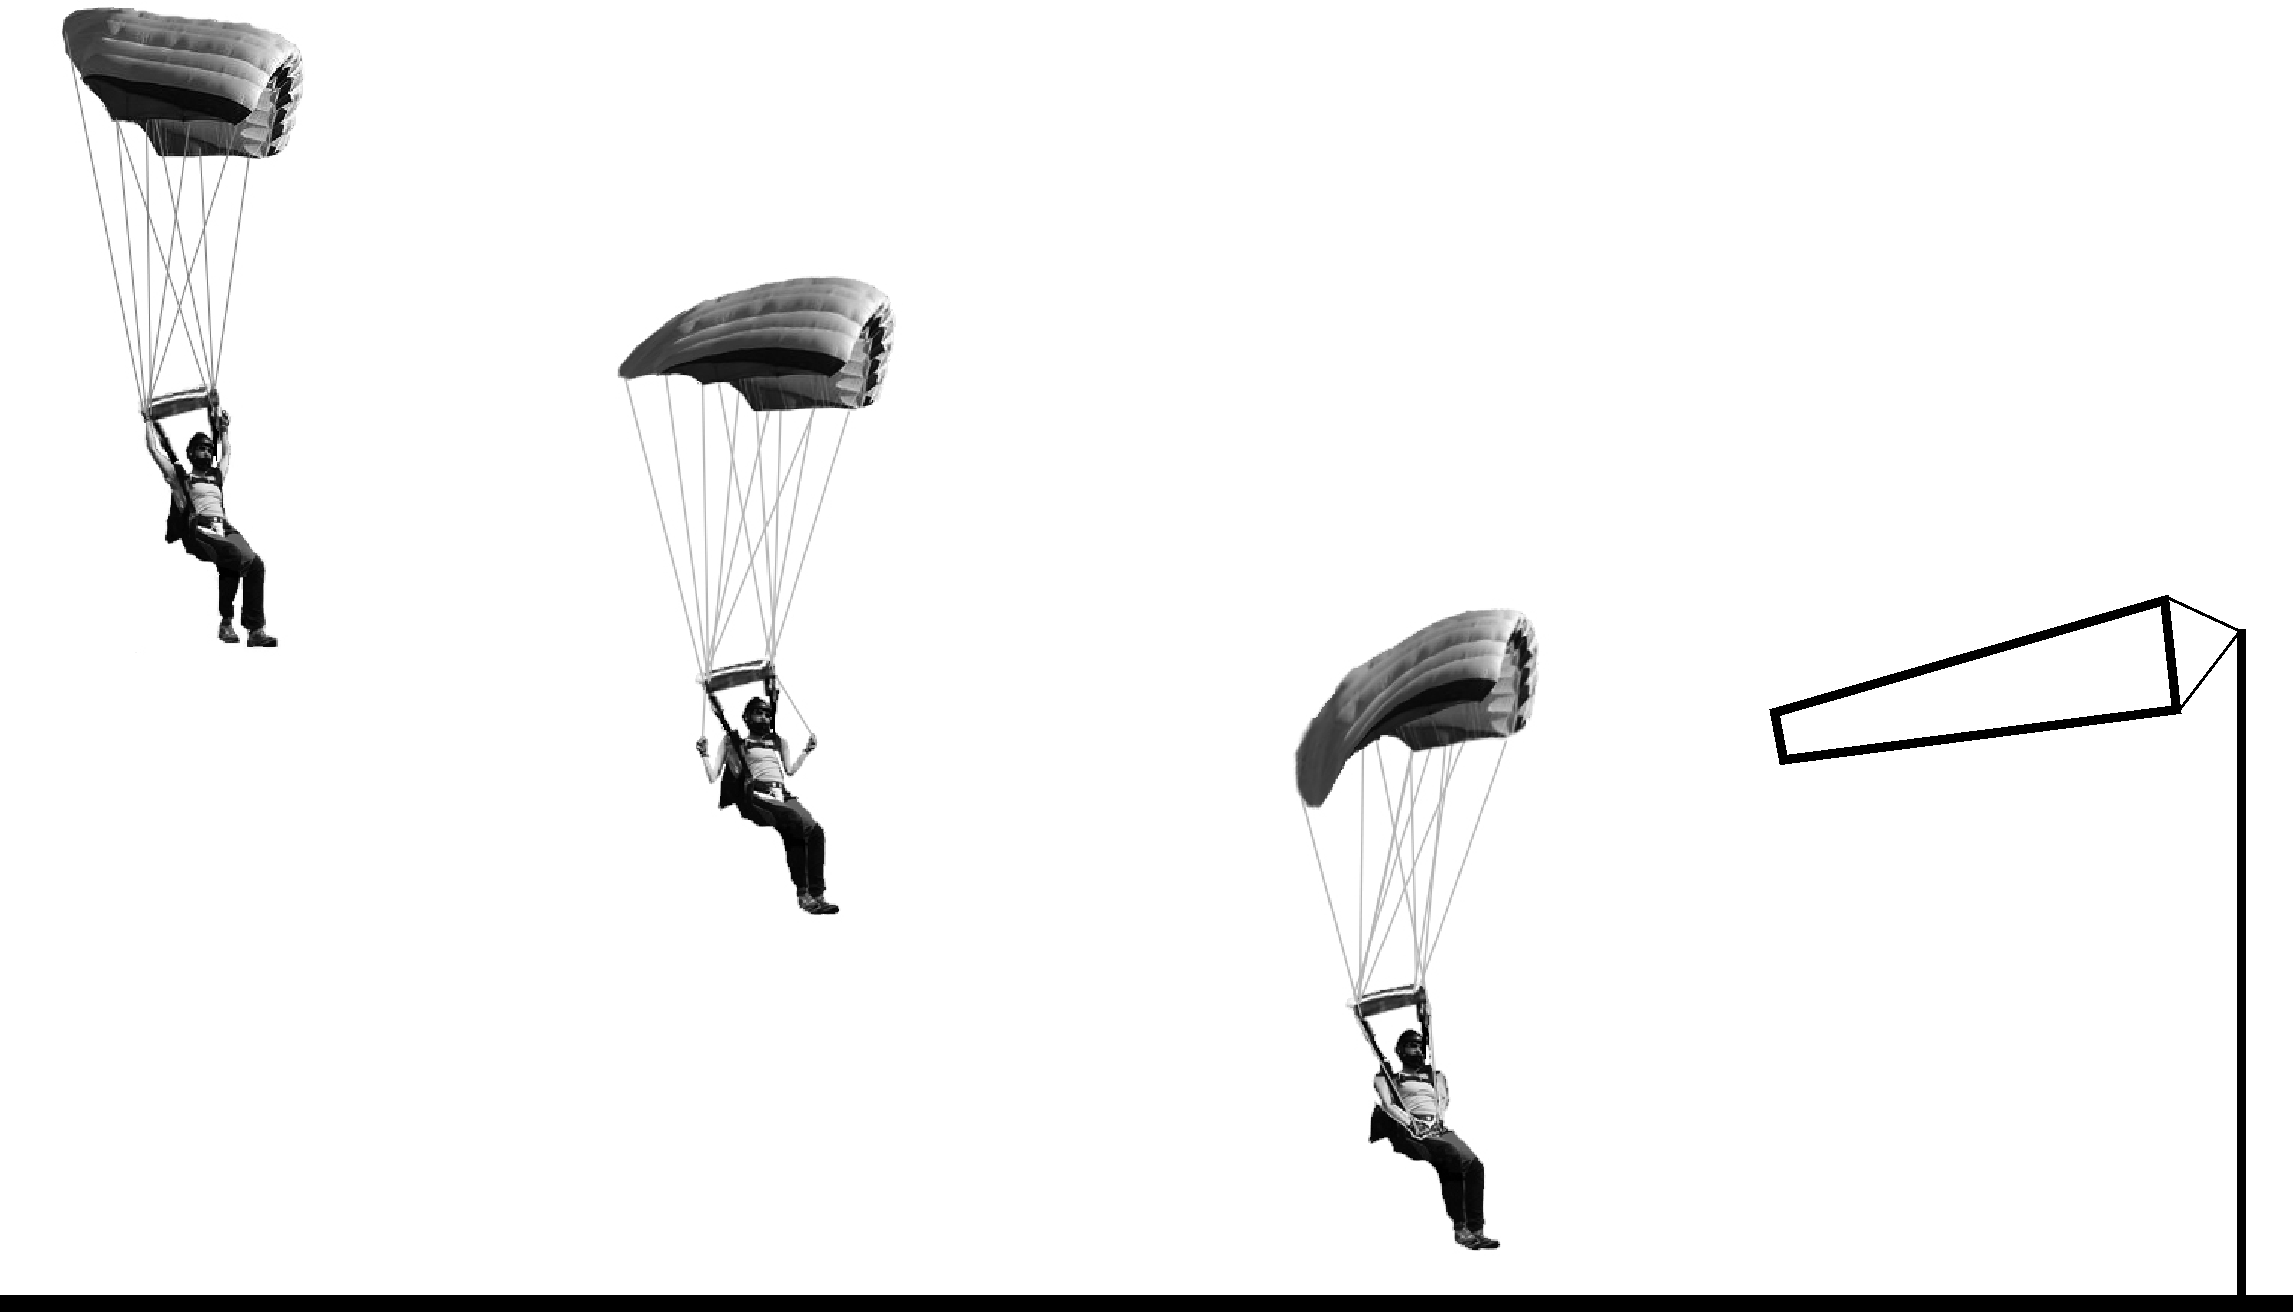
\includegraphics[width=0.6\textwidth]{Loppuveto.png}\caption{Loppuveto}\end{figure*} 


Samalla kun otat alastuloasennon, siirrä ohjauslenkit korvien tasalle. Kun korkeutta on 2-3 metriä, tee loppuveto painamalla ohjauslenkit terävästi täysjarrutustilaan. Ensimmäisillä kolmella hypyllä sinulla on radio, josta kuulet ohjeita esimerkiksi seuraavasti: 

\begin{itemize}
\item  1. hyppy - ohjeita ohjailuun ja laskeutuminen ohjatusti 
\item  2. hyppy - ohjeet tarvittaessa ja laskeutuminen ohjatusti 
\item  3. hyppy - ohjeet vain tarvittaessa 
\end{itemize}

Kun olet noin puiden latvojen tasolla, maa näyttää hyökkäävän silmille. Älä säikähdä, vaan keskity oikeaan alastuloasentoon ja loppuvedon oikeaan ajoitukseen. Korkeuden arvioinnissa voit käyttää apuna esimerkiksi tuulipussin tolppaa, rakennuksen kattoa tai maalialueella olevia ihmisiä.  


Jos teet loppuvedon liian aikaisin ja varjo pysähtyy liian korkealle, \textbf{pidä ohjauslenkit täysjarrutustilassa.} Valmistaudu maahantulokierähdykseen. Jos nostat ohjauslenkit uudelleen ylös, varjo hyökkää eteenpäin ja tulet kovaa maahan. Mikäli et kuule loppuvetokomentoa, niin tee loppuveto itsenäisesti. Jos loppuvedon ajoitus on väärä tai se tehdään huonosti, voi maahantulo olla kova. Tämän vuoksi \textbf{valmistaudu aina tekemään maahantulokierähdys.} 


Suurin osa oppilaiden loukkaantumisista on nilkan nyrjähdyksiä tai murtumia, joista valtaosa olisi vältettävissä hyvän alastuloasennon pitämisellä loppuun saakka. 


Muista aina varjon varassa: 

\begin{itemize}
\item  Tarkkaile ilmatilaa 
\item  Tarkkaile korkeutta 
\item  Vältä rajuja ohjausliikkeitä 
\item  Tarkkaile sijaintiasi ja pysy ohjeistetulla alueella ja suunnitellulla reitillä 
\item  Älä lennä toisen hyppääjän lähellä 
\item  Alempana olevalla on etuajo-oikeus 
\item  Varjo ei käänny hetkessä 
\item  Tarkkaile tuulipussia 
\item  Käänny finaaliin 100 metrissä 
\item  Suora finaali 
\item  Ohjaa varjoa maahan saakka. 
\end{itemize}
\subsection{ Varjon tukahduttaminen }
\label{hyppytapahtuma-varjon-tukahduttaminen}


Kun olet laskeutunut, varjo saattaa hiukan kovemmalla tuulella alkaa vetää sinua perässään. Saat varjon tukahtumaan päästämällä irti toisesta ohjauslenkistä ja vetämällä toisesta kupua luoksesi. Samalla voit juosta varjon toiselle puolelle. Tämä kääntää varjoa niin, ettei tuuli enää pääse täyttämään tunneleita. Aivan viimeisenä keinona voit tehdä päävarjon irtipäästön. (\ref{paavarjon-vajaatoiminnot-varavarjon-kaytto} s.\pageref{paavarjon-vajaatoiminnot-varavarjon-kaytto})  


\textbf{Älä jää maahan makaamaan ellet tarvitse apua.} 


Jos näet hyppääjän vaikeuksissa, velvollisuutesi on auttaa häntä. 

\subsection{ Radiokomennot }
\label{hyppytapahtuma-radiokomennot}


Sinulla on mukanasi radio vähintään kolmella ensimmäisellä hypyllä. Radion tarkoituksena on avustaa sinua ohjaamisessa ja loppuvedon oikea-aikaisessa suorittamisessa. Toimi joka hypyllä itsenäisesti, sillä ohjeita annetaan vain tarvittaessa. Radio on vain apuväline, jossa voi esiintyä häiriöitä. 


1. Yhteyskokeilu ennen koneen kuormausta  


KUTSU = \raisedrule[0.0em]{0.5pt} \\  

\begin{itemize}
\item   Kuittaus kättä nostamalla 
\end{itemize}

2. Yhteyskokeilu ilmassa 


KUTSU + HEILUTA JALKOJA 

\begin{itemize}
\item  Kuittaus jalkojen heilutuksella 
\end{itemize}

3. Käännökset 


KUTSU + VASEN, VASEN, SUORAAN 

\begin{itemize}
\item  Käännä niin kauan, kunnes kuuluu komento SUORAAN 
\end{itemize}

4. Jarruttaminen 


KUTSU + JARRUTA, JARRUTA 

\begin{itemize}
\item  Jokaisella komennolla laske ohjauslenkkejä 10-15 cm 
\end{itemize}

5. Jarrutuksen vähentäminen 


KUTSU + NOSTA, NOSTA 

\begin{itemize}
\item  Jokaisella komennolla nosta ohjauslenkkejä 10-15 cm 
\end{itemize}

KUTSU + LIIDÄ 

\begin{itemize}
\item  Täysliito 
\end{itemize}

6. Itsenäinen ohjaaminen 


KUTSU + OHJAA ITSENÄISESTI 

\begin{itemize}
\item  Jatka ohjaamista itsenäisesti. 
\item  Kumoaa edellisten komentojen vaikutuksen. 
\end{itemize}

7. Loppuveto 


KUTSU + JALAT YHTEEN 

\begin{itemize}
\item  Hyvä alastuloasento, jalat tiukasti yhdessä. 
\end{itemize}

VEDÄ 

\begin{itemize}
\item  Paina ohjauslenkit terävästi täysjarrutustilaan, pidä alastuloasento. 
\end{itemize}
